\documentclass[12pt,onecolumn,a4paper]{article}
\usepackage{epsfig,amsthm,amsmath,booktabs,csquotes}
\usepackage [pagebackref=true, colorlinks, linkcolor=blue, citecolor=magenta, urlcolor=cyan] {hyperref}
\usepackage{color,xcolor}

\usepackage{subcaption}
\usepackage[labelformat=parens,labelsep=quad, skip=3pt]{caption}
\usepackage{graphicx}
\usepackage{enumerate,braket,tcolorbox}
\usepackage[localise]{xepersian}
%\settextfont[Scale=1.2]{‌BNAZANIN.TTF}
%\settextfont[Scale=1.2]{BZAR.TTF}
\settextfont[Scale=1]{XB Niloofar}
\ExplSyntaxOn
\cs_set_eq:NN
\etex_iffontchar:D
\tex_iffontchar:D
\cs_undefine:N \c_one
\int_const:Nn \c_one { 1 }
\ExplSyntaxOff
\setdigitfont[Scale=1]{XB Niloofar}
\setlatintextfont[Scale=1]{Times New Roman}





\begin{document}
\title{مطالعه همگامی در شبکه‌های عصبی} 
\author{محسن مهرانی - استاد راهنما: دکتر سامان مقیمی عراقی}
\date{}
\maketitle
\tableofcontents
\newpage
\قسمت{سخن نخست}
مطالعه فعالیت شبکه‌های عصبی برای تحقیق و بررسی کارکردهای مغز اهمیت زیادی دارد. همه بر این باوریم که مغز محمل اندیشه و تفکر است. ما کنجکاو هستیم که چگونه همکاری بین نورون‌های آن باعث می‌شود تا حافظه، کشف و پردازش صورت گیرد. هر کدام از نورون‌های مغز می‌تواند در حالت فعال [روشن] یا غیرفعال [خاموش] قرار گیرد. هم اکنون شواهدی وجود دارد که کارکردهایی طلایی یاد شده مغز در زمان‌هایی رخ می‌دهند که الگوی خاموش و روشن شدن نورون‌های آن باهم \textbf{«هم‌گامی»} دارند. هم‌گامی به این معناست که جمعیت بزرگی از نورون‌ها هم باهم خاموش و روشن می‌شوند و یک الگوی تکرار شونده‌ای را دنبال می‌کنند. تو گویی که باهم هم‌آهنگ یا هم‌گام شده‌اند.\\

بی‌تردید دستیابی به تمام جزییات مغز برای ما میسّر نیست و به آن به عنوان یک \textbf{«جعبه‌ی سیاه»} نگاه می‌کنیم که مدت‌هاست به دنبال ارائه مدلی هستیم که رابطه‌ی بین ورودی‌ها و خروجی‌های ثبت شده را بازتولید کند. کاری که در این پژوهش انجام خواهیم داد تلاشی است برای پیشنهاد دادن یک مدل برای این جعبه‌ی سیاه که رفتار نسبتا مشابهی را میان ورودی و خروجی‌های این جعبه سیاه و یا مغز ایجاد می‌کند.

\قسمت{مقدمه}
مدل‌های زیادی برای شبکه‌های عصبی ارائه شده است که توانایی تولید رفتار هم‌گام شدن نورون‌ها را در آن‌ها می‌توانیم جستجو کنیم. یکی از این مدل‌ها که در تمام فصول شبیه‌سازی از آغاز تا کنون از آن بهره برده شده است؛ مدل انباشت و شلیک است\cite{PhysRevLett.105.158104}. در این جستار ابتدا با مدل انباشت و شلیک شروع می‌کنیم و سپس مدلی توسعه یافته که آن را \textbf{«چرخنده»} صدا خواهیم کرد؛ می‌پردازیم.\\
متن اصلی این جستار شامل معرفی این مدل‌ها و پویایی آن‌ها در زمان و نتایج ضبط شده از نشانگرهایی است که برای آشکارسازی هم‌گامی تعبیه شده‌اند.

\قسمت{شبکه انباشت و شلیک}
 در این نوشتار \cite{PhysRevLett.105.158104}  نویسندگان تلاش می‌کنند تا هم‌گامی را برای شبکه‌ی نورون‌های مهاری رصد کنند. این نورون‌ها به گونه‌ای باهم مرتبط هستند که تیزه زدن هر نورون منجر به مهار پتانسیل دیگر نورون‌ها می‌شود. تک‌تک نورون‌های این شبکه از تحول انباشت و شلیک تبعیت می‌کند. معادله تحول اختلاف پتانسیل هر کدام از نورون‌ها با محیط بیرونش از رابطه زیر داده می‌شود:
 \begin{tcolorbox}
\begin{align}
\dot{v_i}=a_i - v_i - \frac{g}{N} \sum_{n|t_n<t} S_{i,l(n)} \delta(t - t_n - t_d) 
\label{eq:potential_1}
\end{align}

\begin{enumerate}[-]
\item
$g$: 
ضریب اتصال هر جفت نورون. از آن‌جا که همه‌ی نورون‌ها در این مطالعه مهاری هستند؛ باید این کمیت مثبت انتخاب شود تا تاثیر جمله‌ی پایانی در نهایت منفی باشد.
\item
$S$:
ماتریس همسایگی. این کمیت نشان می‌دهد که آیا دو نورون به هم متصل و تاثیرگذار هستند یا خیر.
\item
$t_d$: 
زمان تاخیر میان زدن تیزه هر نورون و تاثیر آن روی نورون‌های دیگر.
\item
$a_i$:
یک پتانسیل تحریکی و خارجی. در این مطالعه این مقدار برای هر نورون به صورت تصادفی انتخاب می‌شود و تا پایان شبیه‌سازی ثابت باقی می‌ماند.
\item
$N$:
تعداد نورون‌های در شبکه
\end{enumerate}
\end{tcolorbox}
\زیرقسمت{آهنگ تیزه زدن}
پیش از آن که به شبیه‌سازی یک شبکه‌ از نورون‌ها بپردازیم؛ خوب است تا یک نورون تنها را مطالعه کنیم. یک نورون تنها که پویایی از جنس مدل انباشت‌وشلیک دارد؛ دوره تناوب تیزه‌زدن آن از رابطه‌ی زیر قابل محاسبه است .
\begin{align}
\dot{v_i}= I  - v_i &\rightarrow \frac{dv_i}{I - v_i} = dt \\
&\rightarrow T = ln(\frac{I}{I - 1})
\end{align}
این رابطه نشان می‌دهد که بسامد تیزه‌زدن یک نورون با افزایش مجموع جریان‌های ورودی آن به صورت لگاریتمی افزایش می‌یابد.
\زیرقسمت{نشانگر تشخیص فاز هم‌گامی}
برای آن که متوجه شویم که شبکه در حالت هم‌گامی یا ناهم‌گامی است نیاز است تا آشکارسازی را تعبیه کنیم که باتوجه به رفتار سامانه، هم‌گامی یا ناهم‌گامی را با عقربه‌ی خود نشان دهد. برای این منظور ابتدا مفهوم میدان ($E$) را تعریف می‌کنیم که بیانگر شدت فعالیت نورون‌های شبکه است. انحراف از معیار این کمیت در طول زمان، پارامتر مناسبی است که به کمک آن هم‌گامی را تشخیص دهیم.
\begin{tcolorbox}
\begin{align}
\ddot{E}+ 2\alpha \dot{E}+\alpha^{2}E &=\frac{\alpha^2}{N} \sum_{n|tـn<t} \delta(t - t_n - t_d) \\
\sigma^{2} &= \braket{E^{2}}_{t} - \braket{E}^{2}_{t}
\end{align}
*دقت کنیم که شدت میدان با تعداد تیزه زدن‌ها رفتاری ملایم دارد. به عنوان مثال اگر تیزه‌ها متوقف شوند؛ شدت میدان پس از لحظاتی چند [متناسب با $\alpha$] صفر می‌شود.
\end{tcolorbox}

در طول زمان میدان $E$ و $\sigma$ را رصد می‌کنیم. برای دریافت شهودی عملکرد مناسب این پارامتر نظم، فرض کنید که شبکه در حالتی است که جمعیت بزرگی از آن در حال خاموش و روشن شدن هم‌گام است. پس مشاهده خواهم کرد که میدان که شدت فعالیت نورون‌ها را نشان می‌دهد در حال ضربان رفت و برگشتی است. این افت‌وخیز با تقویت هم‌گامی دامنه‌ی بزرگتر پیدا می‌کند به طوری که انحراف آن از میانگین پهنای قابل توجهی کسب می‌کند. از این رو انحراف معیار میدان، کمیت مناسبی است که میزان هم‌گامی را گزارش کند.\\

\subsection{مسائل پیشروی پیاده سازی شبیه سازی}
\subsubsection{تابع بی‌کران دلتا}
یکی از مشکلات شبیه سازی معادلات دیفرانسیلی حضور تابع دلتای دیراک است. این تابع در نقطه صفر خود دارای مقداری بینهایت است. معرفی چنین تابعی به رایانه کاری دشوار است و همانندی محاساتی ندارد. حال برای برطرف کردن این مشکل چه باید کرد؟ نکته در این جا نهفته است که چون ما برای حل عددی معادله دیفرانسیلی خود از زمان پیوسته استفاده نمی‌کنیم و از گام‌هایی با طول مثبت $\Delta t$ استفاده می‌کنیم این مشکل به صورت زیر مدیریت می‌شود.
\begin{align}
v_{i}(t+\Delta t) &= v_{i}(t) + \int_{t}^{t+\Delta t} \dot{v_i}  dt \\
&= v_{i}(t) + \int_{t}^{t+\Delta t} \left[ a_i - v_i - \frac{g}{N} \sum_{n|t_n<t} S_{i,l(n)} \delta(t - t_n - t_d)  \right]   dt \\
&\approx v_{i}(t) +  \left[ a_i - v_i(t) \right] \Delta t - \frac{g}{N} \sum_{n|t_n<t} S_{i,l(n)} \int_{t}^{t+\Delta t} \delta(t - t_n - t_d) dt  \\
&\approx v_{i}(t) +  \left[ a_i - v_i(t) \right] \Delta t - \frac{g}{N} \sum_{n|t_n<t} S_{i,l(n)} H(t + \Delta t- t_n - t_d) \label{eq:potential_changes}
\end{align}

حالا تابع پله کاملا برای ما آشنا و قابل مدلسازی است. دقت شود که تابع پله یاد شده فقط در محدوده $t, t+\Delta t$ زندگی می‌کند و پس از آن اعتبار ندارد. معادله \ref{eq:potential_changes}  می‌گوید که باید برای تحول پتانسیل نورون $i$ام بررسی کنیم که آیا نورونی در همسایگی آن تیزه زده است یا نه. اگر چنان باشد؛ یک واحد به جمع تیزه زدگان اضافه کنیم.


\subsubsection{ثبت تاریخ تیزه زدن‌ها}
برای محاسبه تحول پتانسیل در رابطه \ref{eq:potential_changes} چنان که توضیح داده شد نیاز به دانستن تاریخ تیزه زدن‌ها داریم. اگر بخواهیم برای تمامی نورون‌ها در هر گام زمانی تیزه‌زدن آن را به صورت مجزا ثبت کنیم؛یک آرایه مربعی خواهیم داشت که شماره سطر آن می‌تواند معرف زمان باشد و ستون نماد شماره نورون - شکل شماره (\ref{fig:rasterplot}).\\
\begin{figure}[h]
\centering
  \includegraphics[width = 10 cm]{../scripts/kuramoto_model_synchoronization_problem/single_runs/N1000_T1000_g5_input_1.2_2.8/raster_plot.png}
 \caption{ثبت لحظه‌ای تیزه زدن هر نورون به صورت مجزا - در این نمودار ضریب تاثیر هر نورون روی همسایه‌هایش $g = 5$ بوده است. چنان که انتظار می‌رفت شاهد هم‌گامی هستیم.}
  \label{fig:rasterplot}
\end{figure}
اما مشکلی که برای این شبیه سازی رخ خواهد داد. در صورت افزایش تعداد نورون‌ها و زمان شبیه سازی با یک ابر آرایه روبرو خواهیم شد که امکان دارد در ذخیره سازی آن دچار مشکل شویم. به همین خاطر در شبیه سازی انجام شده تنها مجموع تیزه زدن‌ها را ذخیره کردیم تا یک آرایه یک ستونه داشته باشیم و در ذخیره‌سازی به مشکل نخوریم.

\subsection{نتایج}
اندازه‌ی پارامتر‌هایی که برای این شبیه‌سازی انتخاب کردیم؛ کاملا از صورت مقاله یاد شده برداشته شده و به قرار زیر است.
\begin{tcolorbox}[colback=green!5!white,colframe=green!75!black]
\begin{enumerate}[*]
\item
$\alpha = 20\, s^{-1}$
\item
جریان‌های تصادفی خارجی نورون‌ها از اعضای بازه‌ی $(1.2,2.8)$ انتخاب می‌شوند.
\item
$N = 10000$
\item
$t_d = 0.1\, s$ 
\end{enumerate}
\end{tcolorbox}
این شبیه سازی برای ۱۰۰۰ ثانیه اجرا شده است که در آن هر گام زمانی برابر $0.01$ ثانیه گرفته شده است. کد شبیه‌سازی در پوشه 
\href{run://..//scripts//kuramoto_model_synchoronization_problem}{مسئله همگامی برای مدل انباشت‌و‌شلیک}
قابل مشاهده است.
\زیرزیرقسمت{انحراف از معیار میدان}
مهم‌ترین شاخصه ما برای ردگیری همگامی، انحراف معیار میدان $E$ است که با زیگما $\sigma$ نمایش می‌دهیم. جهش به وجود آمده در شکل‌ (\ref{fig:if_phase_transition}) به این معنی است که سامانه از حالت ناهم‌گامی به هم‌گامی تغییر فاز داده است. 

\begin{figure}[h]
\centering
  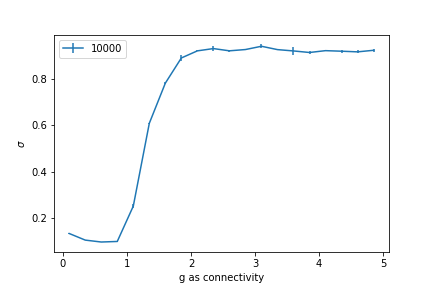
\includegraphics[width = 10 cm]{../papers_studies/figs/IF/sigma.png}
 \caption{تغییر فاز از ناهم‌گامی به هم‌گامی برای ۱۰۰۰ نورون}
  \label{fig:if_phase_transition}
\end{figure}

\زیرزیرقسمت{توزیع تناوب زمانی تیزه‌ها}
شبکه‌ی ما متشکل از نورون‌هایی است که مدام در حال تیزه زدن و فعال نگه‌داشتن شبکه هستند. برخی با بسامد بیشتری تیزه می‌زنند و برخی آهسته‌تر. اگر کنجکاو باشیم که جمعیت کل نورون‌های ما چگونه میان دسته‌های مختلف با تناوب‌های متفاوت توزیع شده‌ است؛ لازم است تا توزیع فراوانی آن‌ها را یکجا رسم کنیم - شکل \ref{fig:if_isi}.\\
همان طور که می‌بینید به ظاهر این توزیع رفتاری توانی دارد و اگر کنجکاو باشیم می‌توانیم شیب این نمودار تمام لگاریتمی آن را جهت محاسبه‌ی نمای توزیع بدست آوریم - شکل \ref{fig:if_isi_trending_line}.
\begin{figure}[h]
\centering
  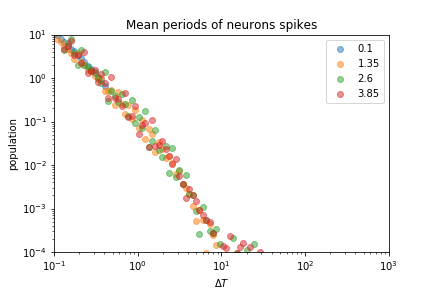
\includegraphics[width = 10 cm]{../papers_studies/figs/IF/mean_spiking_persiods.png}
 \caption{توزیع بسامدی شبکه‌های ۱۰۰۰ نورونی که هر کدام قدرت اتصال متفاوتی دارند. }
  \label{fig:if_isi}
\end{figure}

\begin{figure}[h]
\centering
  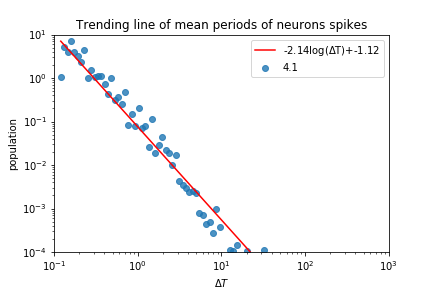
\includegraphics[width = 10 cm]{../papers_studies/figs/IF/mean_spiking_persiods_with_trending_line.png}
 \caption{محاسبه‌ی نمای توزیع توانی فاصله زمانی بین تیزه‌ها}
  \label{fig:if_isi_trending_line}
\end{figure}

\section{شبکه‌ی نورون‌های چرخنده}
در این مدل به جای آن که برای شبکه خود از مدل انباشت-شلیک استفاده کنیم از مدل چرخنده استفاده می‌کنیم. در این مدل نورون‌های ما مانند دونده‌هایی به دور میدان مثلثاتی می‌دوند. ما نقطه‌ی فاز $\pi$ را به عنوان علامت برای این دونده‌ها قرار دادیم. هر زمان که دونده‌ای از علامت خود گذشت یک تیزه برای او درنظرمی‌گیریم و بلافاصله او را به فاز $-\pi$ باز می‌گردانیم.\\

برای توصیف فاز هر نورون از معادلات زیر استفاده می‌کنیم:
\begin{tcolorbox}
\begin{equation}
\begin{cases}
\dot{\theta_i}=I_i - cos(\theta_i) - g E, \hspace{2ex} - 5\pi/2 \leq \theta_i \leq \pi \\
\dot{E} = M - \alpha E\\
\dot{M} = -  \alpha M + \frac{ \alpha^{2} }{N} \sum_{n|tـn<t} \delta(t - t_n - t_d)
\end{cases}
\end{equation}
\begin{enumerate}[-]
\item $\theta_i$:
مشخص کننده‌ی فاز هر نورون. این فاز میان دو لبه در حال حیات است. کوچکترین کران بالای آن همان حالت آستانه در $\pi$ است و بزرگترین کران پایین آن نگه‌دارنده‌ای است که از ریزش نورون‌ها جلوگیری می‌کند.
\item $E$:
میدانی است که شدت فعالیت شبکه را نشان می‌دهد.
\item $M$:
یک پارامتر فرعی که در حل معادله دیفرانسیل مرتبه دوم به دو معادله‌ی تحول مرتبه اول ما را یاری کرده است.
\end{enumerate}
\end{tcolorbox}

این مدل نسبت به مدل قبلی شامل ویژگی‌های مثبتی است. یکی از ویژگی‌های خوب آن این است که پس از بازنشانی فاز نورون تیزه زده، فاز آن به زاویه‌ای برده می‌شود که دارای خواص مثلثاتی مشابهی است. به این معنا که دیگر شاهد گسستگی در اندازه‌ی جملاتی که تحول نورون را توصیف می‌کنند؛ نیستیم.\\
\زیرقسمت{آهنگ تیزه زدن}
برای نورونی تنها که پویایی از جنس چرخنده دارد؛ دوره‌ی تناوب تیزه زدن آن بر حسب مجموع جریان ورودی‌ رفتاری مطابق زیر دارد \cite{safaeesirat2020critical}:

\begin{align}
T = \frac{2\pi}{\sqrt{I^2 - 1}}
\end{align}
این به این معناست که مدل چرخنده و انباشت‌وشلیک اگر چه هر دو با افزایش جریان، بسامد تیزه زدنشان افزایش می‌یابد اما رفتار تغییر آن به دو گونه‌ی متفاوت صورت می‌پذیرد. این نکته‌ی مهمی است که در هنگام مقایسه‌ی دو مدل باید به خاطر داشته باشیم.

\زیرقسمت{نشانگر توسعه یافته‌ی تشخیص همگامی}
برای تشخیص هم‌گامی از یک پارامتر دیگری که در این مقاله \cite{safaeesirat2020critical}  توسط نویسندگان ابداع شده‌است؛ بهره می‌بریم.

\begin{equation}
s =  \braket{ \big[ \frac{1}{N_a}\sum_{i_a} sin(\theta_{i_a}) \big]^{2}}_t
\label{eq:saman_amin_param}
\end{equation}
میانگین‌گیری بالا روی ۱۰۰۰ گام آخر زمانی انجام می‌شود. این فاصله زمانی باید حتما بزرگ‌تر از گام‌های زمانی تحول ریزمقیاس آن باشد. همچنین برای این متوسط‌گیری نورون‌هایی را مدنظر می‌گیریم که در منطقه ی فعال قرار گرفته‌اند. منطقه‌ی فعال، سمت چپ دایره مثلثاتی است.
\subsection{شبیه‌سازی}
ثوابت مسئله را به گونه‌ی زیر انتخاب می‌کنیم.
\begin{tcolorbox}[colback=green!5!white,colframe=green!75!black]
\begin{enumerate}[*]
\item
$\alpha = 20\, s^{-1}$
\item
جریان‌های تصادفی خارجی نورون‌ها از اعضای بازه‌ی $(3.5,13.5)$ انتخاب می‌شوند. این بازه به گونه‌ای انتخاب شده است که یک نورون تنها با دینامیک چرخنده، بسامدی داشته باشد که نورون تنها‌ با دینامیک انباشت‌وشلیک در بازه‌ی $(1.2,2.8)$ داشت.
\item
$N = 10000$
\item
$t_d = 0.1\, s$ 
\end{enumerate}
\end{tcolorbox}
حال شبکه‌ی خود را به ازای قدرت اتصال‌های مختلف اجرا می‌کنیم تا مجددا تحقیق کنیم که چگونه تغییر در قدرت اتصال $g$ می‌تواند باعث شود تا تغییر فاز از ناهم‌گامی به هم‌گامی رخ دهد. برای مشاهده‌ی دفترچه شبیه‌سازی به آدرس 
\href{run://..//scripts//rotational_model}{مسئله همگامی برای مدل چرخنده}
مراجعه کنید.

\subsection{نتایج }
مرتبه‌ی اجرای این الگورتیم خطی است و برای یک شبکه شامل ۱۰۰۰ نورون و برای ۱۰۰۰۰ گام شبیه‌سازی زمانی در حدود ۴ ثانیه به طول می‌انجامد. 


\subsubsection{در جستجوی تغییرفاز}
پس از رصد کردن تغییرات رفتار سیستم بر حسب قدرت مهار نورون‌ها، تغییر فاز مانند مدل قبلی مشاهده شد اما مکان تغییر فاز تغییر کرد و حول $g=30$ قرارگرفت. این تغییر فاز در دو شکل \ref{fig:sigma_rotational} و \ref{fig:amin_saman_rotational}  قابل مشاهده‌است.
\begin{figure}
\centering
  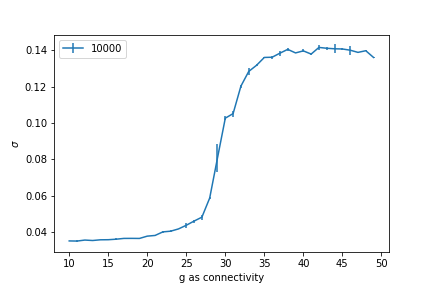
\includegraphics[width = 10 cm]{figs/Rotational/sigma.png}
 \caption{پهنای جریان یک سامانه چرخنده با ده هزار نورون}
  \label{fig:sigma_rotational}
\end{figure}

\begin{figure}
\centering
  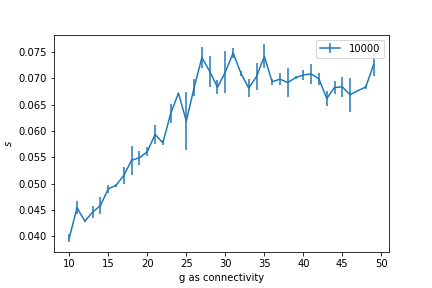
\includegraphics[width = 10 cm]{figs/Rotational/amin_saman_param.png}
 \caption{پارامتر نظم تعریف شده در رابطه \ref{eq:saman_amin_param} برای مدل چرخنده }
  \label{fig:amin_saman_rotational}
\end{figure}

\subsubsection{نورون‌های خاموش}
در حین شبیه‌سازی متوجه شدیم که در ناحیه‌ای که به فاز هم‌گامی در حال گذار هستیم؛ جمعیت نورون‌هایی که همیشه خاموش هستند؛ در حال گسترش است - شکل \ref{fig:silent_neurons_rotational}. هر چه قدر قدرت مهار نورون‌ها را زیاد می‌کنیم؛ این تعداد بیشتر می‌شود. همچنین شایان ذکر است که پس از تغییر فاز این مقدار به اشباع می‌رسد و تعداد نورون‌های فعال به ثبات می‌رسند.
\begin{figure}[h]
\centering
  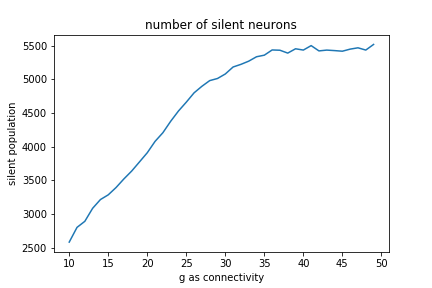
\includegraphics[width = 10 cm]{figs/Rotational/silent_neurons.png}
 \caption{تعداد نورون‌های خاموش برحسب قدرت مهار نورون‌ها}
  \label{fig:silent_neurons_rotational}
\end{figure}

\subsubsection{فاصله زمانی بین تیزه‌ها}
حال که دیدیم برخی نورون‌ها همواره خاموش می‌مانند و یا به عبارتی دوره‌ی تیزه زدن آن‌ها بینهایت است؛ خوب است که دوره‌ی تیزه زدن‌های نورون‌های دیگر را نیز بررسی کنیم. شکل \ref{fig:interspikes_rotational} این شکل نمایان‌گر آن است که توزیع دوره‌ها به توزیع بی‌توانی و رفتار بی‌مقیاس نزدیک است.\\
با این مشاهده، کنجکاو می‌شویم تا نمای بحرانی را برای آن حساب کنیم. در شکل \ref{fig:interspikes_rotational_trending_line} با گذراندن یک خط بر داده‌های بدست آمده از شبکه‌ای با قدرت مهار ۴۵ را می‌بینیم.

\begin{figure}[h]
\centering
  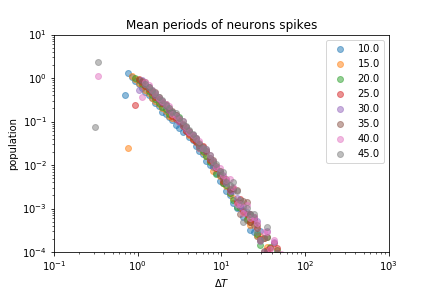
\includegraphics[width = 10 cm]{figs/Rotational/mean_spiking_periods.png}
 \caption{فاصله‌ی زمانی بین تیزه زدن‌ها}
  \label{fig:interspikes_rotational}
\end{figure}

\begin{figure}[h]
\centering
  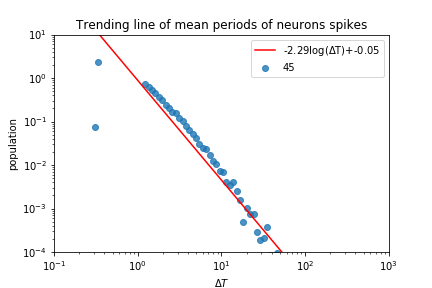
\includegraphics[width = 10 cm]{figs/Rotational/mean_spiking_periods_with_trending_line.png}
 \caption{محاسبه‌ی نمای بحرانی}
  \label{fig:interspikes_rotational_trending_line}
\end{figure}


\subsubsection{فعالیت شبکه}
همان طور که دیدیم تعدادی از نورون‌ها در شبکه به حالت خاموش درمی‌آیند. قابل حدس است که اگر جمعیتی خاموش در شبکه داشته باشیم؛ احتمالا آنهایی هستند که جریان تصادفی اولیه آن‌ها از بقیه کمتر است. برای تحقیق این حدس لازم است تا تعداد تیزه‌های نورون‌های شبکه را بر حسب جریان تصادفی اولیه آنها مرتب کنیم. شکل \ref{fig:spikes_num_vs_background_current} نشانگر سامانه‌ای از ده هزار نورون است که با قدرت $g=50$ روی هم تاثیر می‌گذارند. لازم به ذکر است که این رفتار در فاز هم‌گام قابل مشاهده است. در فاز ناهم‌گام تمام نورون‌ها که از هم تاثیر کمتری می‌پذیرند؛ فعال هستند.


\begin{figure}[h]
\centering
  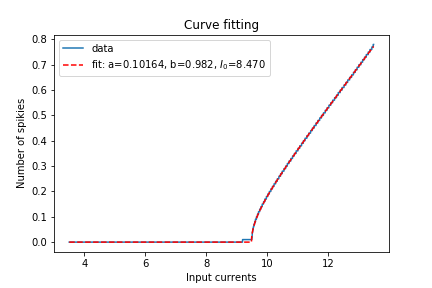
\includegraphics[width = 10 cm]{figs/Rotational/spikies_num_vs_input_fitted_curve_g50_input_3.5_13.5.png}
 \caption{تعداد تیزه بر حسب جریان تصادفی برای سامانه‌ای با ده هزار نورون و ضریب تاثیر $g=50$}
  \label{fig:spikes_num_vs_background_current}
\end{figure}

تعداد تیزه‌های کل شبکه رابطه‌ی مستقیمی با جریان خارجی جاری در شبکه دارد. می‌توانیم با محاسبات تحلیلی نیز به شکل بدست آمده از شبیه‌سازی عددی نزدیک شویم:

\begin{align}
\begin{cases}
I_{in} &= -g \int_{a_{min}}^{a_{max}} p(a) f(a + I_{in}) da \\
f(a) &= \frac{\sqrt{a^2 - 1}}{2\pi}
\end{cases}
\label{eq:analytical_input_current}
\end{align}

در رابطه \ref{eq:analytical_input_current} ، $f(a)$ تابع فعالیت (تعداد تیزه بر ثانیه) تک نورون بر حسب جریان کل ورودی آن است. همچنین $I_{in}$ تمام جریان خارجی جاری در شبکه است.\\
حل این رابطه کمی دشوار است زیرا جریان کل را بر حسب خودش محاسبه کرده است. اما از آنجایی که در انتگرال‌ده تنها یک جابجایی ثابت رخداده است؛ صورت کلی پاسخ انتگرال تغییر نمی‌کند و به صورت زیر بدست خواهد آمد.
\begin{align}
I_{in} = \frac{-g}{2} (-a \sqrt{-1 + a^2} + log(a + \sqrt{-1 + a^2})) \Big|_{a_{min} + I_{in}}^{a_{max} + I_{in}}
\end{align}

\قسمت{تلاش برای توصیف}
حال که دو نوع فاز از سامانه‌ی خود را مشاهده کردیم و هر کدام را به تصویر کشیدیم؛ خوب است در مورد چگونگی گذار از یک حالت به حالت دیگر بحث کنیم. مشخصا باید بپرسیم که چه اتفاقی در سامانه‌ی ما رخ می‌دهد که منجر به تغییر رفتار جریان داخلی $E$ می‌شود. هر کدام از مشخصه‌های این سری زمانی چیست. حول چه میانگینی در حال نوسان است. اندازه‌ی نوسانات آن چقدر است. آیا یک بسامد مشخص دارد؟ یا یک برهم‌نهی از امواج با بسامد‌های متفاوت است.\\

قابل ملاحظه است که در فاز هم‌گام لحظه‌ای وجود دارد که هیچ یک از نورون‌های سامانه تیزه نمی‌زند. به این معنا که در آن لحظه محرکی برای برافروختن میدان $E$ وجود ندارد و زیر پای آن خالی می‌شود.

\زیرقسمت{جریان داخلی در فاز ناهم‌گام}

\زیرقسمت{جریان داخلی در فاز هم‌گام}

\قسمت{شبکه‌ نورون‌های ساده}
حل مسئله‌ی مدل چرخنده‌ بسیار دشوار است و تا تاریخ نوشتن این بند، راه‌حلی تحلیلی برای توصیف گذرفاز آن نیافته‌ایم. علت این موضوع هم حضور جمله‌ی غیرخطی $- cos(\theta)$ در جمله‌ی برهم‌کنش‌های آن‌هاست. حال که با ابعاد دشوار مسئله روبرو شده‌ایم؛ اجازه دهید که زمین بازی خود را عوض کنیم.\\
می‌پرسیم که آیا کیفیت گذرفاز از ناهم‌گامی به هم‌گامی به این جمله وابسته است؟ بی‌تردید پاسخ این سوال را نخواهیم فهمید؛ مگر آن که شبکه‌ی جدیدی مطابق درخواست خود ابداع و شبیه‌سازی کنیم.

\begin{tcolorbox}
\begin{equation}
\begin{cases}
\dot{\theta_i}=I_i  - g E, \hspace{2ex}  \theta_i \leq \pi \\
\dot{E} = M - \alpha E\\
\dot{M} = -  \alpha M + \frac{ \alpha^{2} }{N} \sum_{n|tـn<t} \delta(t - t_n - t_d)
\end{cases}
\end{equation}
\begin{enumerate}[-]
\item $\theta_i$:
مشخص کننده‌ی فاز هر نورون. این فاز میان دو لبه در حال حیات است. کوچکترین کران بالای آن همان حالت آستانه در $\pi$ است و بزرگترین کران پایین آن نگه‌دارنده‌ای است که از ریزش نورون‌ها جلوگیری می‌کند.
\item $E$:
میدانی است که شدت فعالیت شبکه را نشان می‌دهد.
\item $M$:
یک پارامتر فرعی که در حل معادله دیفرانسیل مرتبه دوم به دو معادله‌ی تحول مرتبه اول ما را یاری کرده است.
\end{enumerate}
\end{tcolorbox}

همچنین دقت کنیم که اگر چه این مدل کاهش یافته‌ای از مدل چرخنده است اما در صورت کاستن مدل انباشت‌وشلیک هم به همین جملات برهم‌کنشی می‌رسیدیم. تنها تفاوت در آن می‌شد که فاصله‌ی بین حالت تیزه ($\pi$) و بازنشانی (صفر) در حالت ابداعی $\pi$ برابر مدل کاسته‌شده‌ی انباشت‌وشلیک می‌شد.

\زیرقسمت{شبیه‌سازی}
برای مدل توصیف شده‌ی بالا شبیه‌سازی خود را با تنظیمات زیر به اجرا گذاشتیم. 
\begin{tcolorbox}[colback=green!5!white,colframe=green!75!black]
\begin{enumerate}[*]
\item
$\alpha = 20\, s^{-1}$
\item
جریان‌های تصادفی خارجی نورون‌ها از اعضای بازه‌ی $(9.5,13.5)$ انتخاب می‌شوند.
\item
$N = 10000$
\item
$t_d = 0.1\, s$ 
\end{enumerate}
\end{tcolorbox}

\زیرقسمت{نتایج}
\زیرزیرقسمت{در جستجوی تغییرفاز}
قابل توجه است که کیفیت تغییرفاز با حذف جمله‌ی ذکر شده تغییر نکرد و تنها مکان و ارتفاع انحراف از معیار جریان داخلی است که دست خور تغییر شده است.
\newpage
\bibliographystyle{plain-fa}
\bibliography{MyReferences}

\end{document}


